

\tikzset{every picture/.style={line width=0.75pt}} %set default line width to 0.75pt        

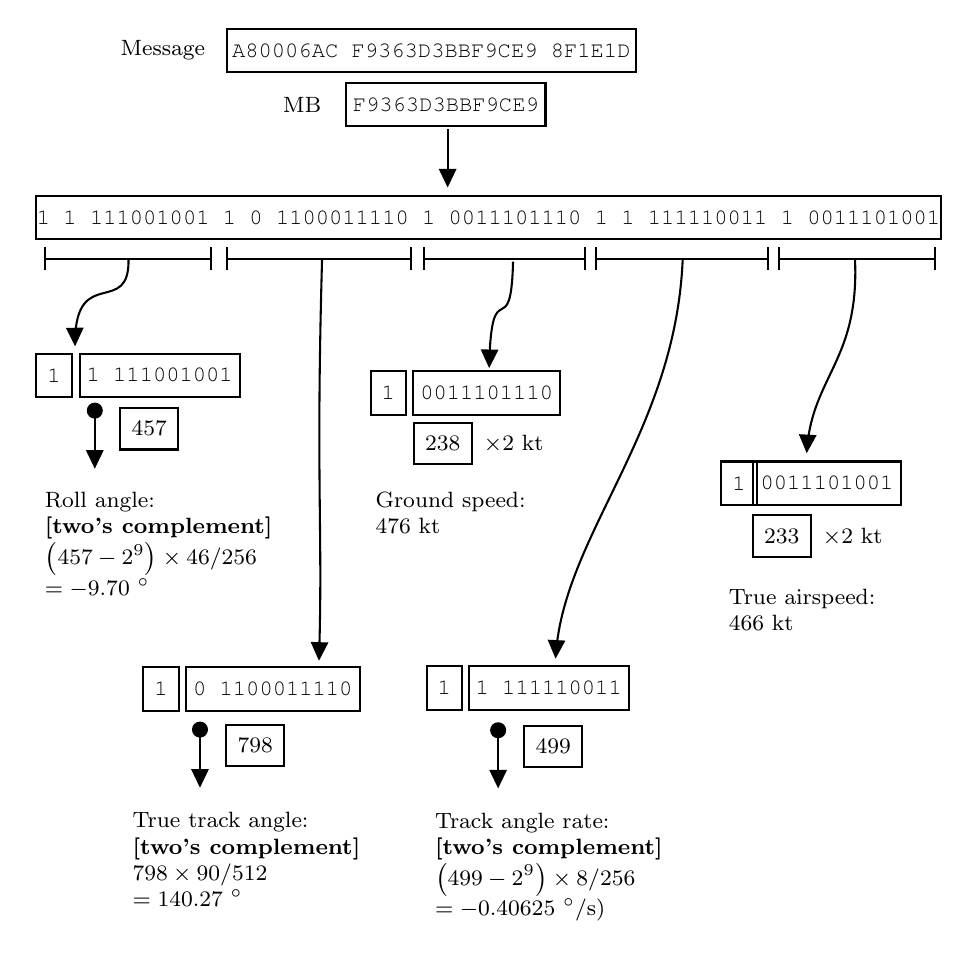
\begin{tikzpicture}[x=0.75pt,y=0.75pt,yscale=-1,xscale=1]
%uncomment if require: \path (0,537); %set diagram left start at 0, and has height of 537

%Curve Lines [id:da05193136470258586] 
\draw    (78.25,134.33) .. controls (78.82,162.77) and (53.17,137.18) .. (52.5,173.58) ;
\draw [shift={(52.5,176.5)}, rotate = 269.06] [fill={rgb, 255:red, 0; green, 0; blue, 0 }  ][line width=0.08]  [draw opacity=0] (8.93,-4.29) -- (0,0) -- (8.93,4.29) -- cycle    ;
%Curve Lines [id:da42930744707627944] 
\draw    (171.5,134.33) .. controls (168.46,242.36) and (171.89,264.35) .. (170.09,325.19) ;
\draw [shift={(170,328)}, rotate = 271.82] [fill={rgb, 255:red, 0; green, 0; blue, 0 }  ][line width=0.08]  [draw opacity=0] (8.93,-4.29) -- (0,0) -- (8.93,4.29) -- cycle    ;
%Curve Lines [id:da6810825834819927] 
\draw    (263.5,135.75) .. controls (262.52,176.91) and (253.38,139.56) .. (252.07,184.17) ;
\draw [shift={(252,187)}, rotate = 271.17] [fill={rgb, 255:red, 0; green, 0; blue, 0 }  ][line width=0.08]  [draw opacity=0] (8.93,-4.29) -- (0,0) -- (8.93,4.29) -- cycle    ;
%Curve Lines [id:da02210524649932588] 
\draw    (428.25,134.33) .. controls (430.44,182.76) and (408.16,190.62) .. (405.19,225.28) ;
\draw [shift={(405,228)}, rotate = 273.09000000000003] [fill={rgb, 255:red, 0; green, 0; blue, 0 }  ][line width=0.08]  [draw opacity=0] (8.93,-4.29) -- (0,0) -- (8.93,4.29) -- cycle    ;
%Straight Lines [id:da8287402060207048] 
\draw [line width=0.75]    (220.5,134.33) -- (298,134.33) ;
\draw [shift={(298,134.33)}, rotate = 180] [color={rgb, 255:red, 0; green, 0; blue, 0 }  ][line width=0.75]    (0,5.59) -- (0,-5.59)   ;
\draw [shift={(220.5,134.33)}, rotate = 180] [color={rgb, 255:red, 0; green, 0; blue, 0 }  ][line width=0.75]    (0,5.59) -- (0,-5.59)   ;
%Straight Lines [id:da6940086335708118] 
\draw [line width=0.75]    (125.5,134.33) -- (214.5,134.33) ;
\draw [shift={(214.5,134.33)}, rotate = 180] [color={rgb, 255:red, 0; green, 0; blue, 0 }  ][line width=0.75]    (0,5.59) -- (0,-5.59)   ;
\draw [shift={(125.5,134.33)}, rotate = 180] [color={rgb, 255:red, 0; green, 0; blue, 0 }  ][line width=0.75]    (0,5.59) -- (0,-5.59)   ;
%Straight Lines [id:da5605080029920126] 
\draw [line width=0.75]    (38,134.33) -- (118,134.33) ;
\draw [shift={(118,134.33)}, rotate = 180] [color={rgb, 255:red, 0; green, 0; blue, 0 }  ][line width=0.75]    (0,5.59) -- (0,-5.59)   ;
\draw [shift={(38,134.33)}, rotate = 180] [color={rgb, 255:red, 0; green, 0; blue, 0 }  ][line width=0.75]    (0,5.59) -- (0,-5.59)   ;
%Straight Lines [id:da26733404149104456] 
\draw [line width=0.75]    (303.5,134.33) -- (386.4,134.33) ;
\draw [shift={(386.4,134.33)}, rotate = 180] [color={rgb, 255:red, 0; green, 0; blue, 0 }  ][line width=0.75]    (0,5.59) -- (0,-5.59)   ;
\draw [shift={(303.5,134.33)}, rotate = 180] [color={rgb, 255:red, 0; green, 0; blue, 0 }  ][line width=0.75]    (0,5.59) -- (0,-5.59)   ;
%Straight Lines [id:da42135663368948384] 
\draw [line width=0.75]    (391.5,134.33) -- (467,134.33) ;
\draw [shift={(467,134.33)}, rotate = 180] [color={rgb, 255:red, 0; green, 0; blue, 0 }  ][line width=0.75]    (0,5.59) -- (0,-5.59)   ;
\draw [shift={(391.5,134.33)}, rotate = 180] [color={rgb, 255:red, 0; green, 0; blue, 0 }  ][line width=0.75]    (0,5.59) -- (0,-5.59)   ;
%Curve Lines [id:da9172630037641052] 
\draw    (345.25,134.33) .. controls (341.88,217.73) and (288.63,266.52) .. (284.17,324.35) ;
\draw [shift={(284,327)}, rotate = 272.90999999999997] [fill={rgb, 255:red, 0; green, 0; blue, 0 }  ][line width=0.08]  [draw opacity=0] (8.93,-4.29) -- (0,0) -- (8.93,4.29) -- cycle    ;
%Straight Lines [id:da508696319168084] 
\draw    (232,72) -- (232,97) ;
\draw [shift={(232,100)}, rotate = 270] [fill={rgb, 255:red, 0; green, 0; blue, 0 }  ][line width=0.08]  [draw opacity=0] (8.93,-4.29) -- (0,0) -- (8.93,4.29) -- cycle    ;
%Straight Lines [id:da38703610180504544] 
\draw    (62,207.5) -- (62,232.5) ;
\draw [shift={(62,235.5)}, rotate = 270] [fill={rgb, 255:red, 0; green, 0; blue, 0 }  ][line width=0.08]  [draw opacity=0] (8.93,-4.29) -- (0,0) -- (8.93,4.29) -- cycle    ;
\draw [shift={(62,207.5)}, rotate = 90] [color={rgb, 255:red, 0; green, 0; blue, 0 }  ][fill={rgb, 255:red, 0; green, 0; blue, 0 }  ][line width=0.75]      (0, 0) circle [x radius= 3.35, y radius= 3.35]   ;
%Straight Lines [id:da8199855675170937] 
\draw    (112.67,361.17) -- (112.67,386.17) ;
\draw [shift={(112.67,389.17)}, rotate = 270] [fill={rgb, 255:red, 0; green, 0; blue, 0 }  ][line width=0.08]  [draw opacity=0] (8.93,-4.29) -- (0,0) -- (8.93,4.29) -- cycle    ;
\draw [shift={(112.67,361.17)}, rotate = 90] [color={rgb, 255:red, 0; green, 0; blue, 0 }  ][fill={rgb, 255:red, 0; green, 0; blue, 0 }  ][line width=0.75]      (0, 0) circle [x radius= 3.35, y radius= 3.35]   ;
%Straight Lines [id:da9593907742960721] 
\draw    (256.33,361.5) -- (256.33,386.5) ;
\draw [shift={(256.33,389.5)}, rotate = 270] [fill={rgb, 255:red, 0; green, 0; blue, 0 }  ][line width=0.08]  [draw opacity=0] (8.93,-4.29) -- (0,0) -- (8.93,4.29) -- cycle    ;
\draw [shift={(256.33,361.5)}, rotate = 90] [color={rgb, 255:red, 0; green, 0; blue, 0 }  ][fill={rgb, 255:red, 0; green, 0; blue, 0 }  ][line width=0.75]      (0, 0) circle [x radius= 3.35, y radius= 3.35]   ;

% Text Node
\draw    (125.63,23.5) -- (322.63,23.5) -- (322.63,44.5) -- (125.63,44.5) -- cycle  ;
\draw (224.13,34) node  [font=\footnotesize] [align=left] {{\fontfamily{pcr}\selectfont A80006AC F9363D3BBF9CE9 8F1E1D}};
% Text Node
\draw (161.88,60) node  [font=\footnotesize] [align=left] {MB};
% Text Node
\draw    (33.7,104) -- (469.7,104) -- (469.7,125) -- (33.7,125) -- cycle  ;
\draw (251.7,114.5) node  [font=\footnotesize] [align=left] {{\fontfamily{pcr}\selectfont 1 1 111001001 1 0 1100011110 1 0011101110 1 1 111110011 1 0011101001}};
% Text Node
\draw    (183.13,49.5) -- (279.13,49.5) -- (279.13,70.5) -- (183.13,70.5) -- cycle  ;
\draw (231.13,60) node  [font=\footnotesize] [align=left] {{\fontfamily{pcr}\selectfont F9363D3BBF9CE9}};
% Text Node
\draw    (33.88,180) -- (50.88,180) -- (50.88,201) -- (33.88,201) -- cycle  ;
\draw (42.38,190.5) node  [font=\footnotesize] [align=left] {{\fontfamily{pcr}\selectfont 1}};
% Text Node
\draw    (54.76,180) -- (131.76,180) -- (131.76,201) -- (54.76,201) -- cycle  ;
\draw (93.26,190.5) node  [font=\footnotesize] [align=left] {{\fontfamily{pcr}\selectfont 1 111001001}};
% Text Node
\draw    (74.26,206.25) -- (102.26,206.25) -- (102.26,226.25) -- (74.26,226.25) -- cycle  ;
\draw (88.26,216.25) node  [font=\footnotesize] [align=left] {457};
% Text Node
\draw    (85.38,331) -- (102.38,331) -- (102.38,352) -- (85.38,352) -- cycle  ;
\draw (93.88,341.5) node  [font=\footnotesize] [align=left] {{\fontfamily{pcr}\selectfont 1}};
% Text Node
\draw    (105.76,331) -- (189.76,331) -- (189.76,352) -- (105.76,352) -- cycle  ;
\draw (147.76,341.5) node  [font=\footnotesize] [align=left] {{\fontfamily{pcr}\selectfont 0 1100011110}};
% Text Node
\draw    (125.26,358.92) -- (153.26,358.92) -- (153.26,378.92) -- (125.26,378.92) -- cycle  ;
\draw (139.26,368.92) node  [font=\footnotesize] [align=left] {798};
% Text Node
\draw    (194.88,188.5) -- (211.88,188.5) -- (211.88,209.5) -- (194.88,209.5) -- cycle  ;
\draw (203.38,199) node  [font=\footnotesize] [align=left] {{\fontfamily{pcr}\selectfont 1}};
% Text Node
\draw    (215.3,188.5) -- (286.3,188.5) -- (286.3,209.5) -- (215.3,209.5) -- cycle  ;
\draw (250.8,199) node  [font=\footnotesize] [align=left] {{\fontfamily{pcr}\selectfont 0011101110}};
% Text Node
\draw    (215.6,213.25) -- (243.6,213.25) -- (243.6,233.25) -- (215.6,233.25) -- cycle  ;
\draw (229.6,223.25) node  [font=\footnotesize] [align=left] {238};
% Text Node
\draw (248,223.75) node [anchor=west] [inner sep=0.75pt]  [font=\footnotesize] [align=left] {$\displaystyle \times 2$ kt};
% Text Node
\draw (94.82,34) node  [font=\footnotesize] [align=left] {Message};
% Text Node
\draw    (363.88,232) -- (380.88,232) -- (380.88,253) -- (363.88,253) -- cycle  ;
\draw (372.38,242.5) node  [font=\footnotesize] [align=left] {{\fontfamily{pcr}\selectfont 1}};
% Text Node
\draw    (379.3,232) -- (450.3,232) -- (450.3,253) -- (379.3,253) -- cycle  ;
\draw (414.8,242.5) node  [font=\footnotesize] [align=left] {{\fontfamily{pcr}\selectfont 0011101001}};
% Text Node
\draw    (221.88,330.67) -- (238.88,330.67) -- (238.88,351.67) -- (221.88,351.67) -- cycle  ;
\draw (230.38,341.17) node  [font=\footnotesize] [align=left] {{\fontfamily{pcr}\selectfont 1}};
% Text Node
\draw    (242.2,330.67) -- (319.2,330.67) -- (319.2,351.67) -- (242.2,351.67) -- cycle  ;
\draw (280.7,341.17) node  [font=\footnotesize] [align=left] {{\fontfamily{pcr}\selectfont 1 111110011}};
% Text Node
\draw (92.76,272.17) node  [font=\footnotesize] [align=left] {Roll angle:\\\textbf{[two's complement]}\\$\displaystyle \left( 457-2^{9}\right) \times 46/256$\\$\displaystyle =-9.70\ ^{\circ }$};
% Text Node
\draw (233.42,256.67) node  [font=\footnotesize] [align=left] {Ground speed:\\476 kt};
% Text Node
\draw (135.09,423.83) node  [font=\footnotesize] [align=left] {True track angle:\\\textbf{[two's complement]}\\$\displaystyle 798\times 90/512$\\$\displaystyle =140.27\ ^{\circ }$};
% Text Node
\draw    (268.92,359.25) -- (296.92,359.25) -- (296.92,379.25) -- (268.92,379.25) -- cycle  ;
\draw (282.92,369.25) node  [font=\footnotesize] [align=left] {499};
% Text Node
\draw (280.76,427.5) node  [font=\footnotesize] [align=left] {Track angle rate:\\\textbf{[two's complement]}\\$\displaystyle \left( 499-2^{9}\right) \times 8/256$\\$\displaystyle =-0.40625\ ^{\circ }$/s)};
% Text Node
\draw    (378.93,257.92) -- (406.93,257.92) -- (406.93,277.92) -- (378.93,277.92) -- cycle  ;
\draw (392.93,267.92) node  [font=\footnotesize] [align=left] {233};
% Text Node
\draw (411.33,268.42) node [anchor=west] [inner sep=0.75pt]  [font=\footnotesize] [align=left] {$\displaystyle \times 2$ kt};
% Text Node
\draw (402.76,303.33) node  [font=\footnotesize] [align=left] {True airspeed:\\466 kt };


\end{tikzpicture}